\subsection{Проектирование и разработка сервиса-координатора}
\label{sec:design:server}

\subsubsection{} Этапы разработки программного средства
\label{sec:design:server:overview}

Архитектурный стиль разделения функциональности программной системы на уровни поднимает сразу несколько проблем. 
Их решение в типичном случае заключается в выполнении следующих этапов~\cite{application_architecture_guide}:

\begin{enumerate}
	\item определение стратегии разбиения на уровни;
	\item определение уровней;
	\item распределение функциональности по уровням и компонентам;
	\item уточнение количества уровней: при необходимости некоторые из них объединяются;
	\item установление правил взаимодействия уровней;
	\item идентификация функциональности, которая используется на всех\linebreak уровнях (cross cutting concerns);
	\item определение интерфейсов уровней;
	\item выбор стратегии развертывания;
	\item выбор конкретных протоколов взаимодействия.
\end{enumerate}

К данному этапу разработки дипломного проекта выполнены шаги с \ref{sec:design:server:overview}а по \ref{sec:design:server:overview}д. 
Шаг \ref{sec:design:server:overview}е вследствие использования различных программных средств, применяемых на уровнях, будет выполняться позднее -- на соответствующих уровнях.

Таким образом, следующий этап -- это определение интерфейсов уровней.
Предполагается, что инициатором любых действий будет являться клиентская часть программного средства. 
Следовательно, единственный интерфейс, который следует определить -- это интерфейс сервиса-координатора части.

Как правило веб-сервисами пользуется большое количество людей одновременно, поэтому при проектировании необходимо учесть данный фактор и реализовать
автономность и независимость частей проектируемой системы. Именно по этой причине был выбран сервис-ориентированный архитектурный стиль.

\subsubsection{} Программный интерфейс сервиса-координатора
\label{sec:design:server:interface}

Предварительным условием для проектирования серверной части приложения является определение его интерфейса в высокоуровневых терминах предметной области. 
Таким образом, далее приведены методы его API, которые основаны на функциональных требованиях, определенных в подразделе~\ref{sec:domain:specification}:

\begin{itemize}
    \item метод создания игрового лобби;
    \item метод подключения к игровому лобби;
    \item метод отключения от игрового лобби;
    \item метод выполнения игровых комманд;
    \item метод получения списка игровых лобби.
\end{itemize}

На рисунке~\ref{fig:design:server:interface:service_alg} приведена схема алгоритма обработки запросов перечисленных методов программного интерфейса серверной частью приложения. 
Далее приведены архитектурные решения, которые были применены при реализации данной части программной системы. 

\begin{sidewaysfigure}
\centering
	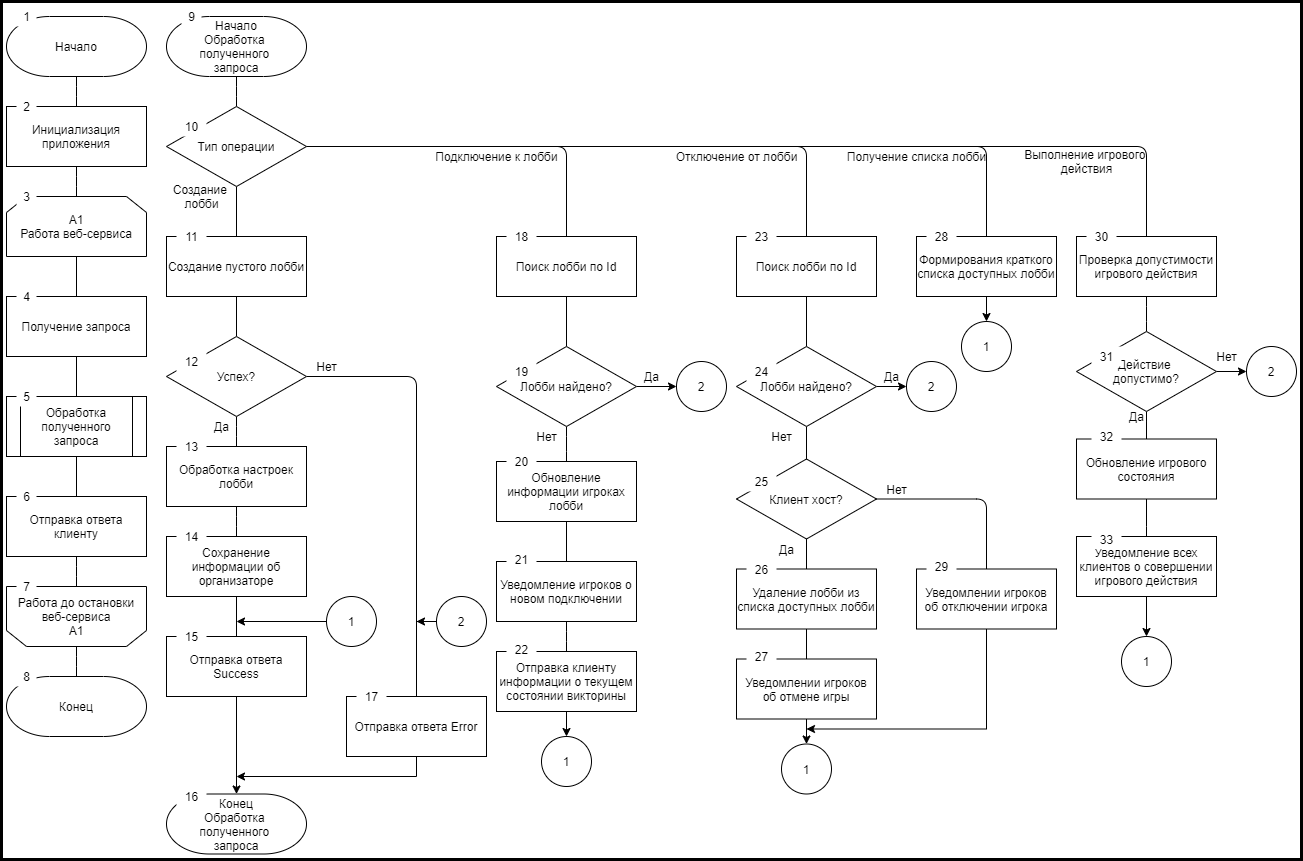
\includegraphics[scale=0.7]{attachments/service_alg.png}
	\caption{Схема программы серверной части программного средства}
	\label{fig:design:server:interface:service_alg}
\end{sidewaysfigure}


Следует отметить, что доступ к методам веб-сервиса может получить любой желающий, использующий протокол TCP и знающий конечную точку для подключения, 
в том числе разработчик альтернативного клинта для игры, например, для мобильных телефонов.
Поэтому разработанный подход является максимально гибким с точки зрения дальнейшего расширения программного средства, а также поддержки кроссплатформенности.

\subsubsection{} Выбор протоколов коммуникации
\label{sec:design:server:protocols}

В пункте~\ref{sec:design:server:overview} приведены этапы, в соответствии с которыми рекомендуется производить проектирование программного 
системы~\cite{application_architecture_guide}. Этап \ref{sec:design:server:overview}з будет рассмотрен позднее вследствие неоднородности и 
отсутствия схожести в применяющихся технологий между уровнями. Таким образом, следующий актуальный этап -- \ref{sec:design:server:overview}и: выбор 
конкретных протоколов взаимодействия.

Можно выделить два основных протокола, которые (с необходимыми дополнениями в каждом конкретном случае) применяются в информационных системах, 
содержащих веб-сервисы~\cite{application_architecture_guide}: TCP (Transmission control protocol -- протокол управления передачей данных) и 
UDP (User datagram protocol -- протокол пользовательский дейтаграм). Они оба используются для передачи данных от клиента серверу и обратно.

Основное отличие между данными протоколами состоит в способе передачи данных. UDP является протоколом передачи данных без установки соединения, в таком случае
данные могуть не достичь адресата. Этот протокол является более быстрым по сравнению с TCP, в то время как надежность значительно меньше. Этот протокол используется
в приложениях, где точность данных не слишком важна или, где объем пересылаемых данных за единицу времени достаточно большой.

Протокол TCP является более надежным по сравнению с UDP, перед отправкой пакетов необходимо установить соединение, качество которого проверяется через систему трех рукопожатий.
Такой подход гарантирует высокую целостность данных при более низкой скорости их передачи. Скорость теряется в процессе пересылки служебных данных, отвечающих за целостность, в то
время как полезные данные ждут своей очереди.

В данном приложении используется TCP, так как для выполнения команд необходима высокая точность передаваемых данных, а сами данные пересылаются не очень часто.
